%% Chapter 3 — Hardware Platform
\section{Hardware Platform}
\label{sec:hardware}

\subsection{Xilinx ZCU216 RFSoC}

The Xilinx Zynq UltraScale+ ZCU216 evaluation board~\cite{ZCU216} is built around an RFSoC
device that integrates, on a single chip, a quad-core ARM Cortex-A53 processor,
an FPGA fabric, and 16 RF-DAC and 16 RF-ADC channels with sampling rates up to
\SI{9.85}{\giga S/s} and \SI{2.5}{\giga S/s}, respectively.  At 14-bit resolution,
the converters can directly synthesise and capture signals in the
\SIrange{0}{6}{\giga\hertz} range without an external frequency up-conversion stage,
provided the analogue signal chain is suitably conditioned.

The ZCU216 was chosen for practical reasons rather than as a bespoke control
instrument.  It is a general-purpose RFSoC evaluation board, commercially available
and of the kind a laboratory can readily obtain, and it is one of the platforms
supported by \QICK{}, the open-source control framework at the centre of this work
(Section~\ref{subsec:qick_stack}).  \QICK{} is also moving from a research tool
toward a commercially supported standard: in 2026 the US Department of Energy and
Fermilab finalised an agreement for the control-electronics vendor Qblox to
commercialise and distribute it~\cite{QbloxQICK2026}.  Other RFSoC boards would
also run \QICK{}; the ZCU216 is the one that was available for this project.

The board runs the PYNQ Linux distribution, which exposes the FPGA fabric and the
converters through Python libraries, making it straightforward to implement and
iterate on firmware/software stacks.  Table~\ref{tab:zcu216} summarises the key
specifications relevant to this thesis.

\begin{table}[ht]
      \centering
      \caption{Selected ZCU216 specifications relevant to qubit readout.}
      \label{tab:zcu216}
      \begin{tabular}{lll}
            \toprule
            Parameter        & Value                 & Note              \\
            \midrule
            DAC channels     & 16                    & Differential GSPS \\
            DAC rate         & up to \SI{9.85}{GS/s} & Per channel       \\
            DAC resolution   & 14 bit                &                   \\
            ADC channels     & 16                    & Differential GSPS \\
            ADC rate         & up to \SI{2.5}{GS/s}  & Per channel       \\
            ADC resolution   & 14 bit                &                   \\
            FPGA fabric      & UltraScale+           & 930k LUT          \\
            Processor        & 4$\times$ Cortex-A53  & \SI{1.5}{GHz}     \\
            Operating system & PYNQ Linux            &                   \\
            \bottomrule
      \end{tabular}
\end{table}

\subsection{QICK Software and Firmware}
\label{subsec:qick_stack}

The Quantum Instrumentation Control Kit (\QICK)~\cite{Stefanazzi2022,QICK_github} is an
open-source framework originally developed at Fermilab that turns an RFSoC board
into a self-contained qubit controller.  It consists of two layers:

\paragraph{Firmware.}
The digital logic loaded onto the FPGA, built from reusable hardware modules
(\emph{IP blocks}) using Vivado, AMD/Xilinx's FPGA design software.  Vivado
compiles a description of the desired logic into a \emph{bitstream}, the
configuration file that programs the FPGA fabric into the required circuit at
power-on.  The \QICK{} firmware comprises:
\begin{itemize}
      \item \textbf{Signal generators}: DDS-based waveform engines that drive the
            DACs with arbitrary envelopes, constant tones, or flat-top pulses.
            Generator 0 (the \texttt{axis\_signal\_gen\_v6} engine, DAC tile 2 block 0)
            is used as the primary readout generator throughout this work.
      \item \textbf{Readout blocks}: ADC-side DDS demodulators that down-convert the
            received signal to baseband.  Each readout block provides both a decimated
            output (time-domain I/Q waveform) and an accumulation buffer (averaged I/Q
            pair).  Readout channel 0 (ADC tile 2 block 0) receives the returning tone.
      \item \textbf{tProcessor V2}: a soft-processor that orchestrates pulse timing
            with nanosecond precision.  It executes a custom instruction set including
            direct memory writes (\texttt{memri}), register arithmetic (\texttt{mathi},
            \texttt{regwi}), conditional branches (\texttt{condj}), and pulse triggers.
            The ZCU216 uses the 64-bit variant of the tProcessor, which extends the
            original 32-bit design with wider arithmetic and richer branching.
\end{itemize}

\paragraph{Software.}
A Python library (the \texttt{qick} package) that runs on the ARM core and
exposes high-level classes for writing and running experiments:
\begin{itemize}
      \item \texttt{QickSoc}: instantiates the full hardware stack, loads the
            bitstream, and provides access to the converters and tProcessor.
      \item \texttt{AveragerProgramV2} (from \texttt{qick.asm\_v2}): the base class
            for measurement sequences on the tProcessor-V2 firmware used here.  A
            program subclasses it and defines \texttt{\_initialize()}, which declares
            the generators and readouts and registers named pulses, and
            \texttt{\_body()}, which plays those pulses, triggers the readout, and
            advances time with \texttt{delay\_auto()}.  Parameter sweeps run either
            inside the FPGA via \texttt{add\_loop()} or across separately compiled
            programs from a Python loop (Section~\ref{subsec:spectroscopy}).
\end{itemize}

In this work the board was accessed over SSH and driven from Jupyter notebooks
running in the on-board PYNQ environment, which is how all the experiments
reported here were carried out.

\subsection{XM655 Analogue Front-End Module}
\label{subsec:xm655}

The ZCU216's RF converters use differential signalling on High-Density (HD)
headers (the DAC and ADC used here sit on JHC3 and JHC7).  The XM655 module is Xilinx's daughter-card
solution: it provides BALUN (balanced-to-unbalanced) transformers that convert the
differential DAC outputs and ADC inputs to/from single-ended SMA ports, along with
optional filtering.

The key constraint introduced by the XM655 in this work is its bandwidth: the
BALUNs cover \SIrange{10}{6000}{\mega\hertz}, so resonator frequencies above
\SI{6}{\giga\hertz} require connections directly on the HD header pins using pigtail
cables.  Those tones also fall in the DAC's second Nyquist zone, so the generator is
run with \texttt{nqz=2} to synthesise them; this, together with the balun rolloff,
is why the highest resonators are reached by bypassing the XM655 baluns.

The loopback path used for calibration experiments consists of:
DAC tile 2 blk 0 (JHC3) $\to$ HD-SMA pigtail $\to$ BALUN $\to$ SMA cable
$\to$ BALUN $\to$ HD-SMA pigtail $\to$ ADC tile 2 blk 0 (JHC7).

Figure~\ref{fig:system_topology} shows the high-level signal flow from the
tProcessor to the qubit chip and back.

\begin{figure}[t]
      \centering
      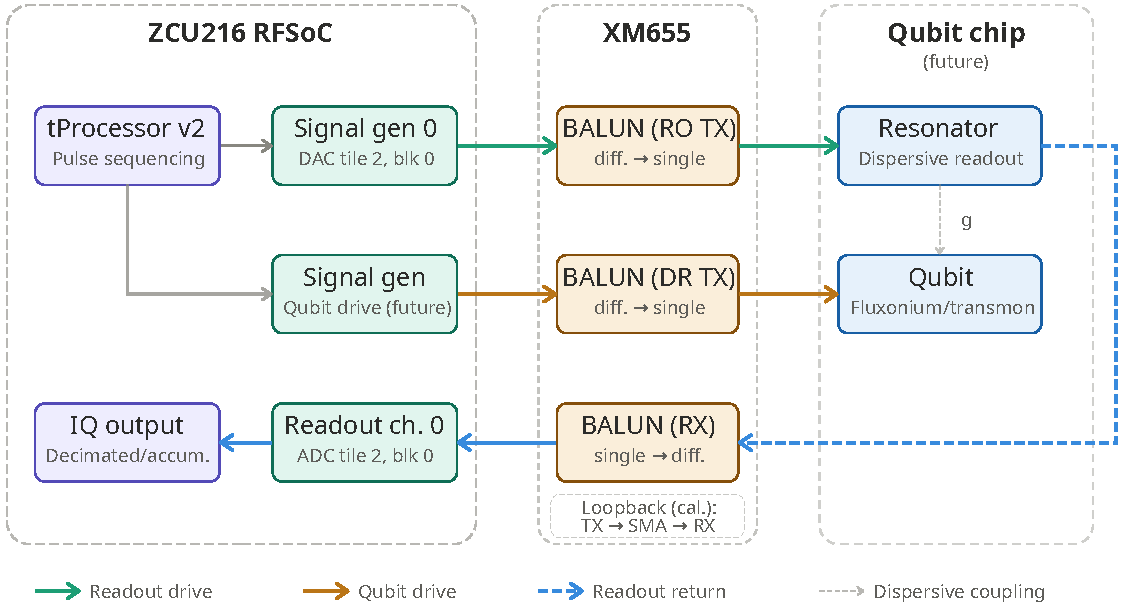
\includegraphics[width=0.92\columnwidth]{figures/system_topology}
      \caption{System signal chain for the \QICK{}-based readout platform.  The
            tProcessor V2 sequences pulses on two generator channels: the readout
            generator drives the readout tone through the XM655 TX BALUN to the
            resonator, and a second generator drives the qubit directly via a second
            TX BALUN channel for $\pi$-pulse control.  The reflected readout tone
            returns through the XM655 RX BALUN to the readout ADC and is demodulated
            to an IQ pair (the channel and port numbers are those of
            Table~\ref{tab:channels}).  The XM655 BALUNs cover
            \SIrange{10}{6000}{\mega\hertz}; resonator frequencies above
            \SI{6}{\giga\hertz} require direct HD-header pigtail connections,
            bypassing the XM655.  The qubit chip and its connections are shown as a
            design target; the board was not connected to a qubit chip within the
            scope of this work.  Calibration experiments use the loopback path
            (TX~BALUN $\to$ SMA cable $\to$ RX~BALUN) shown inside the XM655
            container.}
      \label{fig:system_topology}
\end{figure}
